\documentclass[11pt]{article}
\usepackage[utf8]{inputenc}	% Para caracteres en español
\usepackage{amsmath,amsthm,amsfonts,amssymb,amscd}
\usepackage{multirow,booktabs}
\usepackage[table]{xcolor}
\usepackage{fullpage}
\usepackage{lastpage}
\usepackage{enumitem}
\usepackage{fancyhdr}
\usepackage{mathrsfs}
\usepackage{wrapfig}
\usepackage{setspace}
\usepackage{calc}
\usepackage{multicol}
\usepackage{cancel}
\usepackage[retainorgcmds]{IEEEtrantools}
\usepackage[margin=1cm]{geometry}
\usepackage{amsmath}
\newlength{\tabcont}
\setlength{\parindent}{0.0in}
\setlength{\parskip}{0.05in}
\usepackage{empheq}
\usepackage{framed}
\usepackage[most]{tcolorbox}
\usepackage{xcolor}
\usepackage{graphicx}
\usepackage{listings}
% -- Basic formatting
\usepackage[utf8]{inputenc}
\usepackage[english]{babel}
\usepackage{times}
\usepackage{caption}
\usepackage{subcaption}
\usepackage{placeins}
\setlength{\parindent}{0pt}
\usepackage{indentfirst}% -- Defining colors:
\usepackage[dvipsnames]{xcolor}
\definecolor{codegreen}{rgb}{0,0.6,0}
\definecolor{codegray}{rgb}{0.5,0.5,0.5}
\definecolor{codepurple}{rgb}{0.58,0,0.82}
\definecolor{backcolour}{rgb}{0.95,0.95,0.92}% Definig a custom style:
\lstdefinestyle{mystyle}{
    backgroundcolor=\color{backcolour},   
    commentstyle=\color{codepurple},
    keywordstyle=\color{NavyBlue},
    numberstyle=\tiny\color{codegray},
    stringstyle=\color{codepurple},
    basicstyle=\ttfamily\footnotesize\bfseries,
    breakatwhitespace=false,         
    breaklines=true,                 
    captionpos=t,                    
    keepspaces=true,                 
    numbers=left,                    
    numbersep=5pt,                  
    showspaces=false,                
    showstringspaces=false,
    showtabs=false,                  
    tabsize=2
}% -- Setting up the custom style:
\lstset{style=mystyle}
\lstset{
  style=mystyle,
  framexleftmargin=3.5mm,
  rulesepcolor=\color{black},
  linewidth=0.6\linewidth,
  xleftmargin=12pt,
  aboveskip=12pt,
  belowskip=12pt
}
\colorlet{shadecolor}{orange!15}
\parindent 0in
\parskip 1pt
\geometry{margin=1in, headsep=0.25in}
\theoremstyle{definition}
\newtheorem{defn}{Definition}
\newtheorem{reg}{Rule}
\newtheorem{exer}{Exercise}
\newtheorem{note}{Note}
\graphicspath{ {./images/} }
\begin{document}
\setcounter{section}{0}
\title{MIE223 Lecture Notes}

\thispagestyle{empty}

\begin{center}
{\LARGE \bf Basic NLP Text Processing}\\
{\large MIE223}\\
Winter 2025
\end{center}
\section{Basic NLP Text Processing.
 NLP=Natural Language Processing}
\subsection{NLP Text Processing Pipeline}
nltk provides
implementations
for most operations

\begin{itemize}
  \item Document → Sections and Paragraphs
  \item Paragraphs → Sentences (sentence segmentation / extraction)
  \item Sentences → Tokens
  \item Tokens → Lemmas or Morphological Variants / Stems
  \item Tokens → Part-of-speech (POS) Tags
  \item Tokens, POS Tags → Phrase Chunks (Noun \& Verb Phrases)
  \item Tokens, POS Tags → Parse Trees
  \begin{itemize}
    \item Augment above with coreference, entailment, sentiment, ...
  \end{itemize}
\end{itemize}

\section{Basic Text
Processing: Word tokenization}
\subsection{Text Normalization}
Every NLP task needs to do text
normalization:
\begin{enumerate}
  \item Segmenting/tokenizing words in running text
  \item Normalizing word formats
  \item Segmenting sentences in running text
\end{enumerate}

\subsection{How many words?}
I do uh main- mainly business data processing

\begin{itemize}
  \item Fragments, filled pauses
\end{itemize}

Seuss’s cat in the hat is different from other cats

\begin{itemize}
  \item Lemma: same stem, part of speech, rough word sense
  \item cat and cats = same lemma
  \item Wordform: the full inflected surface form
  \item cat and cats = different wordforms
\end{itemize}

they lay back on the San Francisco grass and looked at the stars and their

\begin{itemize}
  \item Type: an element of the vocabulary.
  \item Token: an instance of that type in running text.
  \item How many? Depends on how you segment. San Francisco can be one token
  \begin{itemize}
    \item 15 tokens (or 14)
    \item 13 types (or 12) (or 11?)
  \end{itemize}
\end{itemize}

\begin{equation}
  N = \text{number of tokens} 
\end{equation}
\begin{equation}
  V = \text{vocabulary} = \text{set of types} 
\end{equation}
\begin{equation}
  |V| = \text{size of vocabulary}
\end{equation}
\begin{equation}
  |V| > O(N^{1/2})
\end{equation}

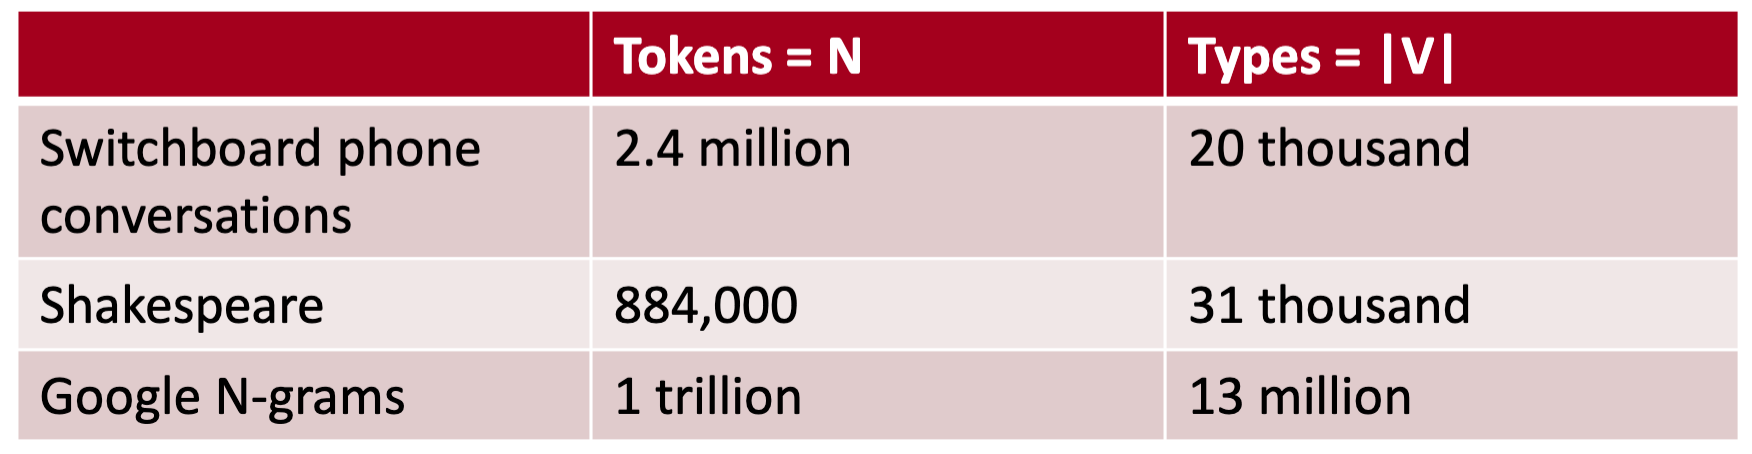
\includegraphics[width=\textwidth]{1.png}

\subsection{Issues in Tokenization}

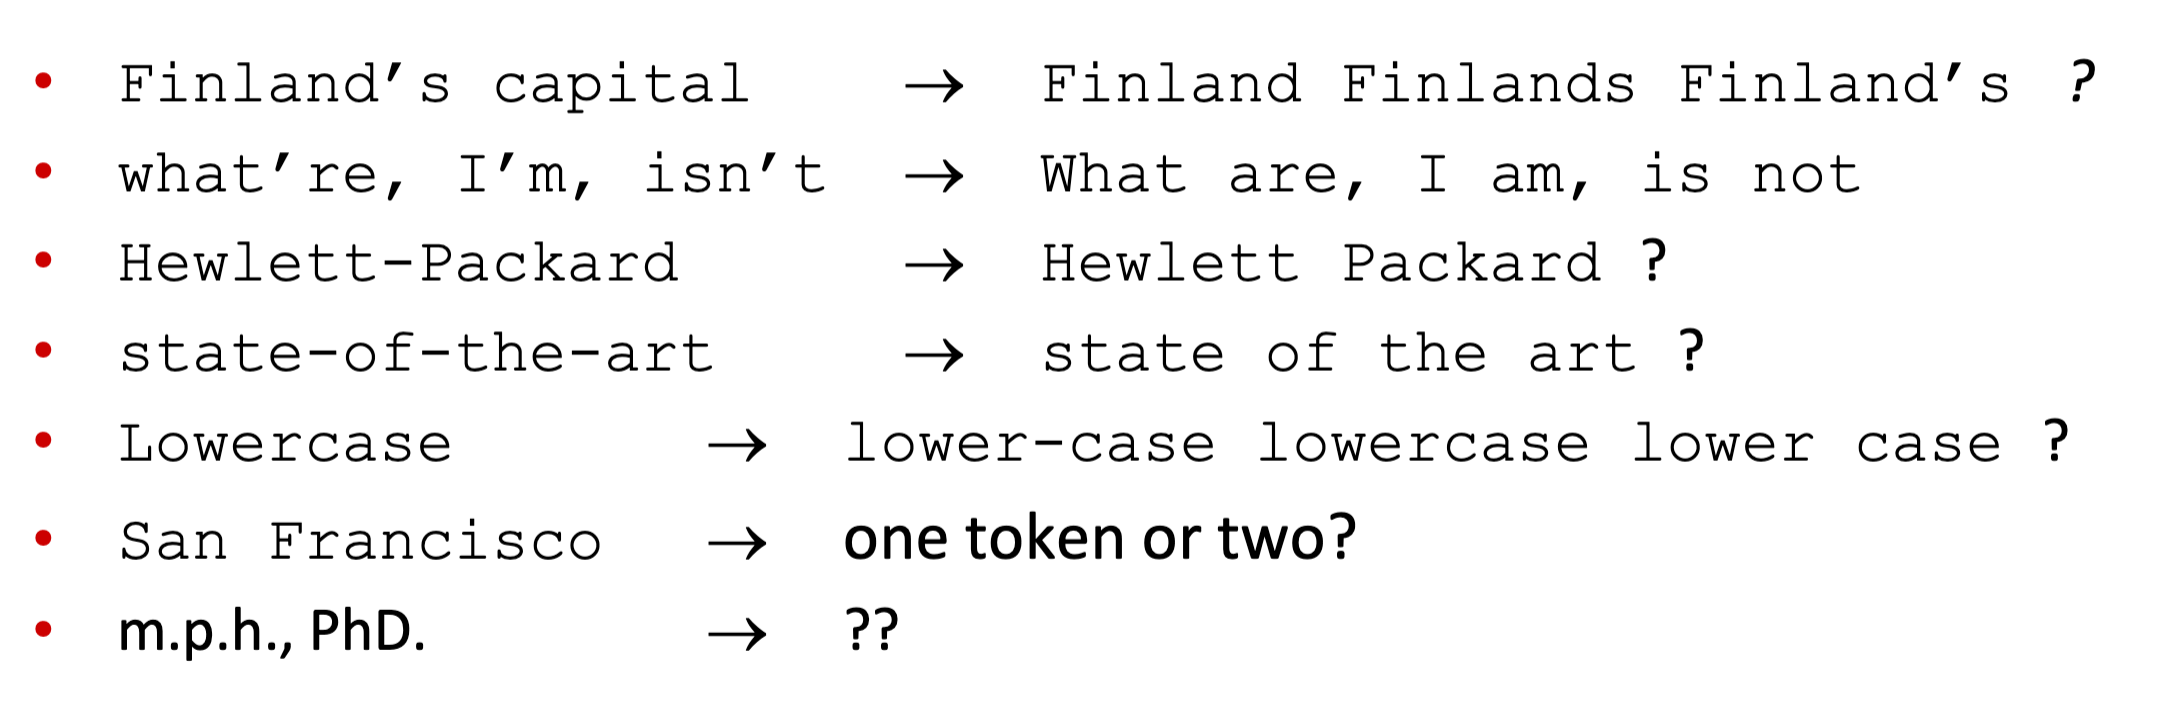
\includegraphics[width=\textwidth]{2.png}

Keep hyphens together? Remove contractions? Does upper and lower case matter?

\subsection{Tokenization: language issues}
\begin{itemize}
  \item French
  \item L'ensemble → one token or two?
  \item L ? L’ ? Le ?
  \item Want l’ensemble to match with un ensemble
  \item German noun compounds are not segmented
  \item Lebensversicherungsgesellschaftsangestellter
  \item ‘life insurance company employee’
  \item German information retrieval needs compound splitter
\end{itemize}

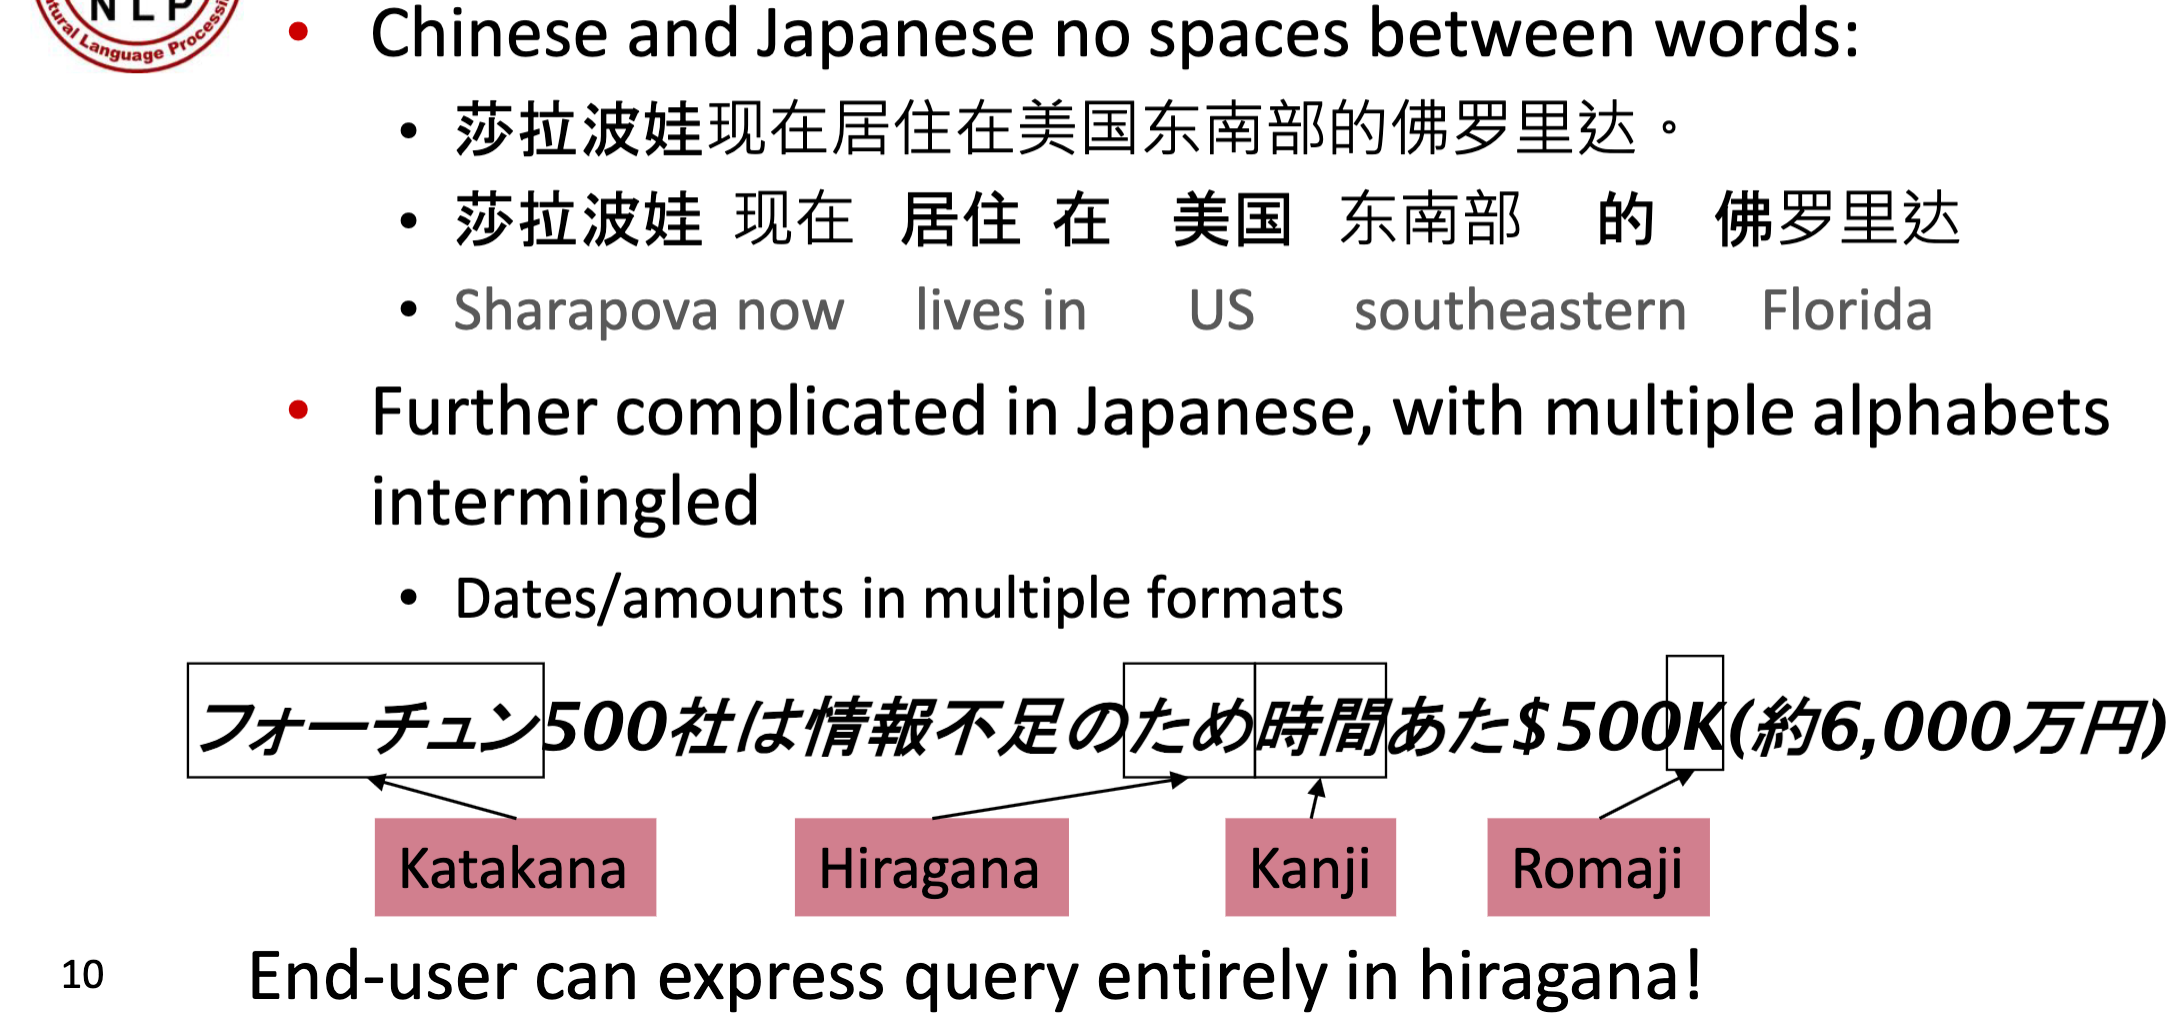
\includegraphics[width=\textwidth]{3.png}

\section{Word Normalization and
Stemming}
\subsection{Normalization}
\begin{itemize}
  \item Need to “normalize” terms
  \begin{itemize}
    \item Information Retrieval: indexed text \& query terms must have same form.
    \begin{itemize}
      \item We want to match U.S.A. and USA
    \end{itemize}
  \end{itemize}
  \item We implicitly define equivalence classes of terms
  \begin{itemize}
    \item e.g., deleting periods in a term
  \end{itemize}
  \item Alternative: asymmetric expansion:
  \begin{itemize}
    \item Enter: window Search: window, windows
    \item Enter: windows Search: Windows, windows, window
    \item Enter: Windows Search: Windows
  \end{itemize}
  \item Potentially more powerful, but less efficient
\end{itemize}

\subsection{Case folding}
\begin{itemize}
  \item Applications like IR: reduce all letters to lower case
  \begin{itemize}
    \item Since users tend to use lower case
    \item Possible exception: upper case in mid-sentence?
    \begin{itemize}
      \item e.g., General Motors
      \item Fed vs. fed
      \item SAIL vs. sail
    \end{itemize}
  \end{itemize}
  \item For sentiment analysis, MT, Information extraction
  \begin{itemize}
    \item Case is helpful (US versus us is important)
  \end{itemize}
\end{itemize}

\subsection{Lemmatization}
\begin{itemize}
  \item Reduce inflections or variant forms to base form
  \begin{itemize}
    \item am, are, is → be
    \item car, cars, car's, cars' → car
  \end{itemize}
  \item the boy's cars are different colors → the boy car be different color
  \item Lemmatization: have to find correct dictionary headword form
  \item Machine translation
  \begin{itemize}
    \item Spanish quiero (‘I want’), quieres (‘you want’) same lemma as querer ‘want’
  \end{itemize}
\end{itemize}

\subsection{Morphology}
\begin{itemize}
  \item Morphemes:
  \begin{itemize}
    \item The small meaningful units that make up words
    \item Stems: The core meaning-bearing units
    \item Affixes: Bits and pieces that adhere to stems
    \begin{itemize}
      \item Often with grammatical functions
    \end{itemize}
  \end{itemize}
\end{itemize}

\subsection{Stemming}
\begin{itemize}
  \item Reduce terms to their stems in information retrieval
  \item Stemming is crude chopping of affixes
  \begin{itemize}
    \item language dependent
    \item e.g., automate(s), automatic, automation all reduced to automat.
  \end{itemize}
  \item for example compressed
  and compression are both
  accepted as equivalent to
  compress. → for exampl compress and
  compress ar both accept
  as equival to compress
\end{itemize}

\subsection{Porter’s algorithm: 
The most common English stemmer}
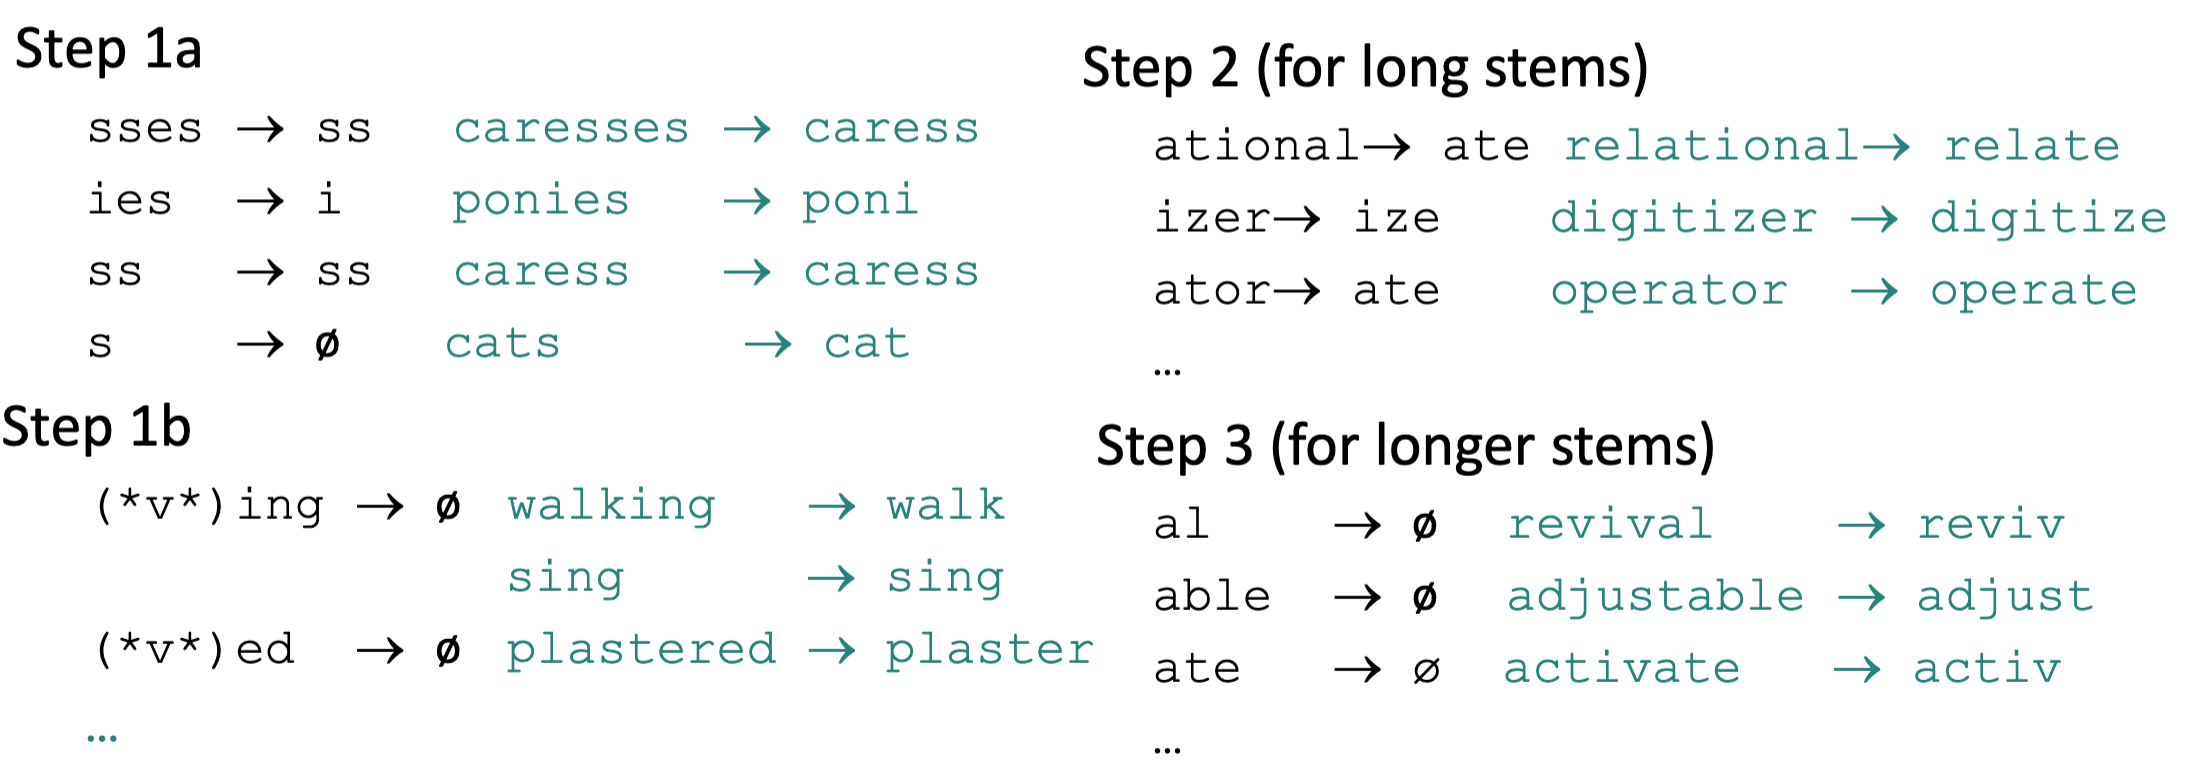
\includegraphics[width=\textwidth]{4.png}

\subsection{Viewing morphology in a corpus
Why only strip –ing if there is a vowel?}

(*v*)ing → ø walking → walk
sing → sing

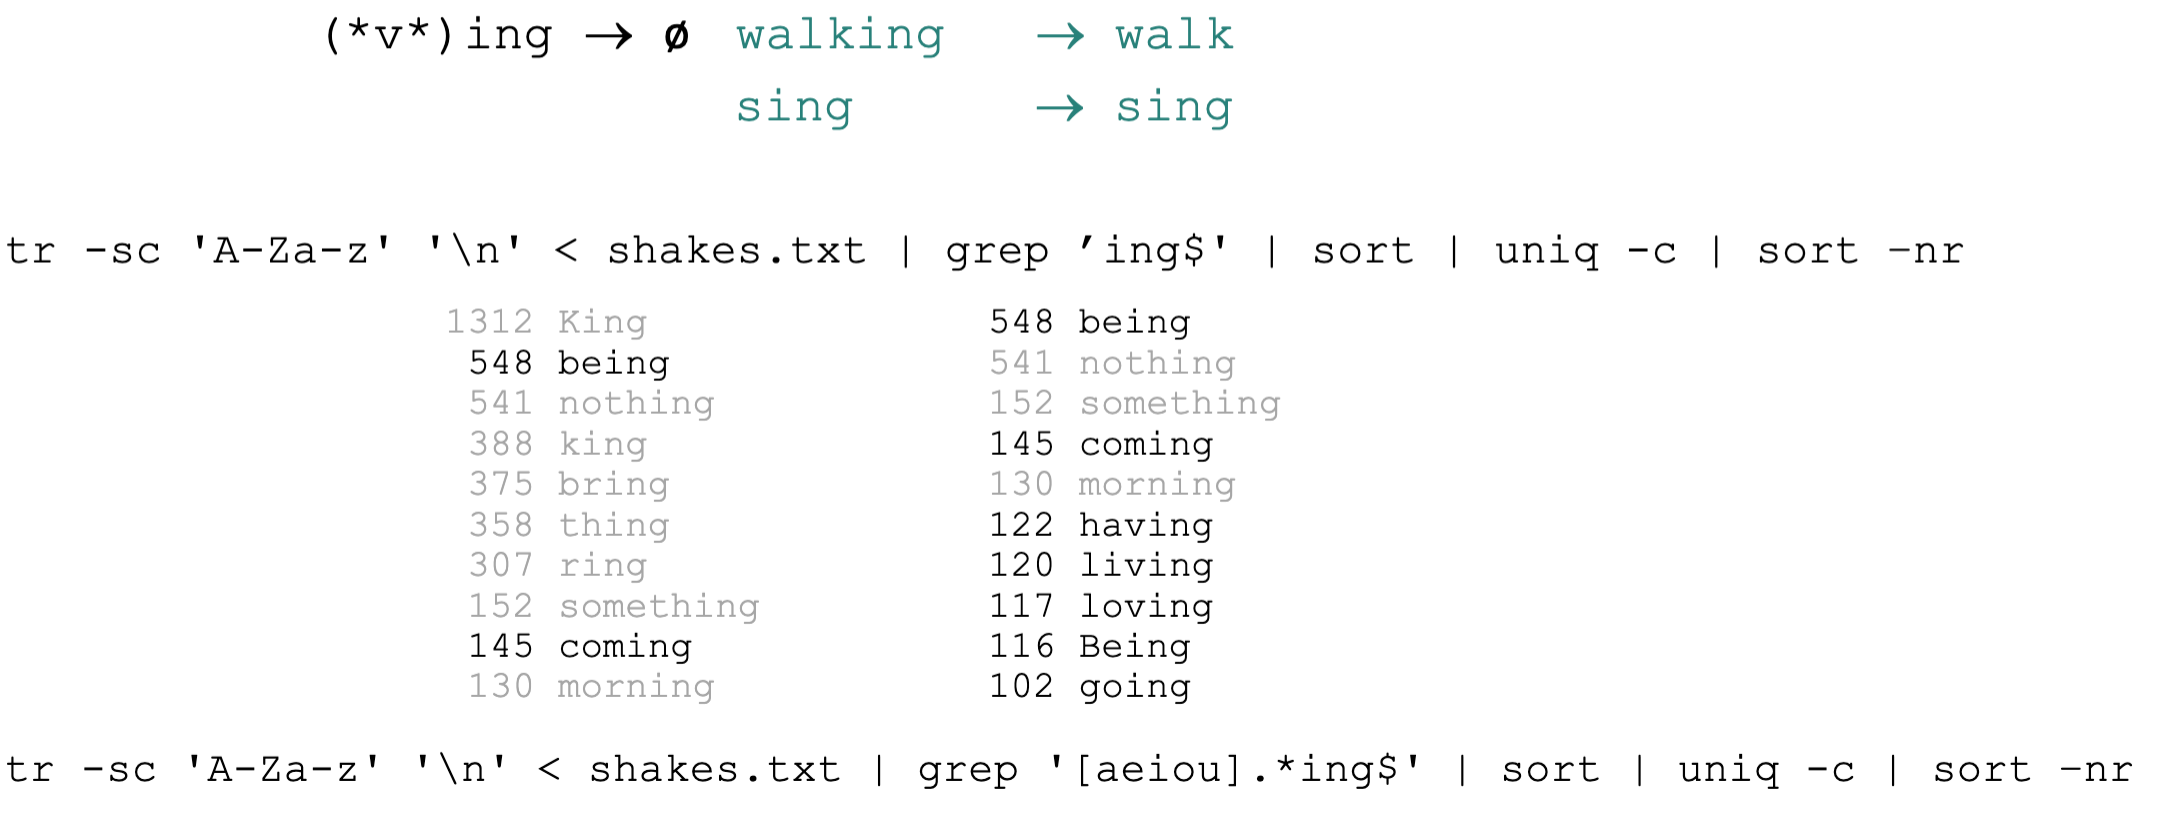
\includegraphics[width=\textwidth]{5.png}

\subsection{Dealing with complex morphology is
sometimes necessary}
\begin{itemize}
  \item Some languages requires complex morpheme segmentation
  \item Turkish
  \item Uygarlastiramadiklarimizdanmissinizcasina
  \item `(behaving) as if you are among those whom we could not civilize’
  \item Uygar `civilized’ + las `become’
  \item tir `cause’ + ama `not able’
  \item dik `past’ + lar ‘plural’
  \item imiz ‘p1pl’ + dan ‘abl’
  \item mis ‘past’ + siniz ‘2pl’ + casina ‘as if’
\end{itemize}

\section{Sentence Segmentation
and Decision Trees}
\subsection{Sentence Segmentation}
\begin{itemize}
  \item !, ? are relatively unambiguous
  \item Period “.” is quite ambiguous
  \begin{itemize}
    \item Sentence boundary
    \item Abbreviations like Inc. or Dr.
    \item Numbers like .02\% or 4.3
  \end{itemize}
  \item Build a binary classifier
  \item f(input) = {True, False}
  \item "The car is traveling 10 m.p.h." 
  \item Check which period is ending the sentence
  \begin{itemize}
    \item Looks at a “.”
    \item Decides EndOfSentence/NotEndOfSentence
    \item Classifiers: hand-written rules, regular expressions, or machine-learning
  \end{itemize}
\end{itemize}

\subsection{Determining if a word is end-of-sentence:
a Decision Tree}
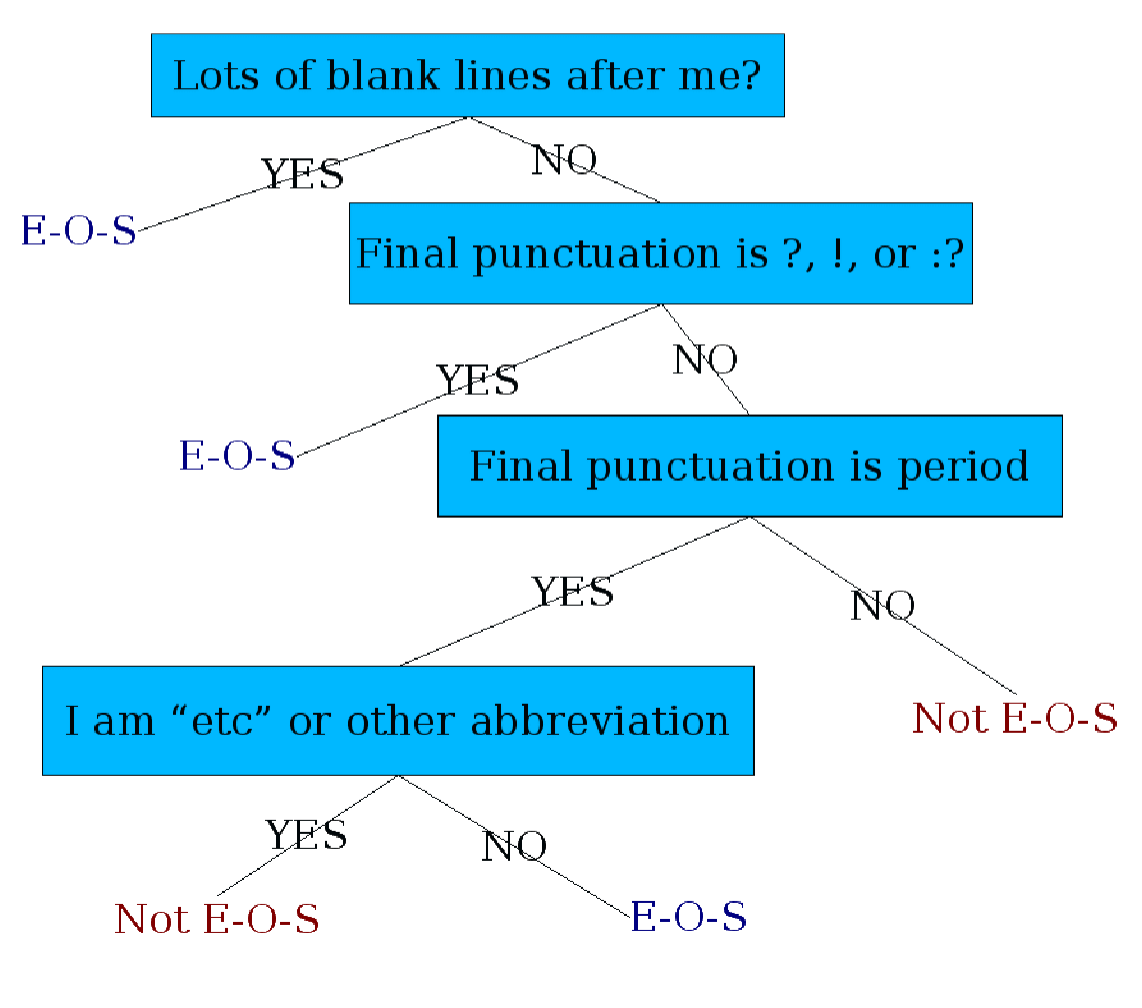
\includegraphics[width=\textwidth/2]{6.png}
\subsection{More sophisticated decision tree features}
\begin{itemize}
  \item Case of word with “.”: Upper, Lower, Cap, Number
  \item Case of word after “.”: Upper, Lower, Cap, Number
  \item Numeric features
  \begin{itemize}
    \item Length of word with “.”
    \item Probability(word with “.” occurs at end-of-s)
    \item Probability(word after “.” occurs at beginning-of-s)
  \end{itemize}
\end{itemize}

\section{Regular
Expressions:
Detecting word
pattern variations}
\subsection{Regular expressions}
\begin{itemize}
  \item A formal language for specifying text strings
  \item How can we search for any of these?
  \begin{itemize}
    \item woodchuck
    \item woodchucks
    \item Woodchuck
    \item Woodchucks
  \end{itemize}
\end{itemize}

\subsection{Regular Expressions: Disjunctions}
Letters inside square brackets []

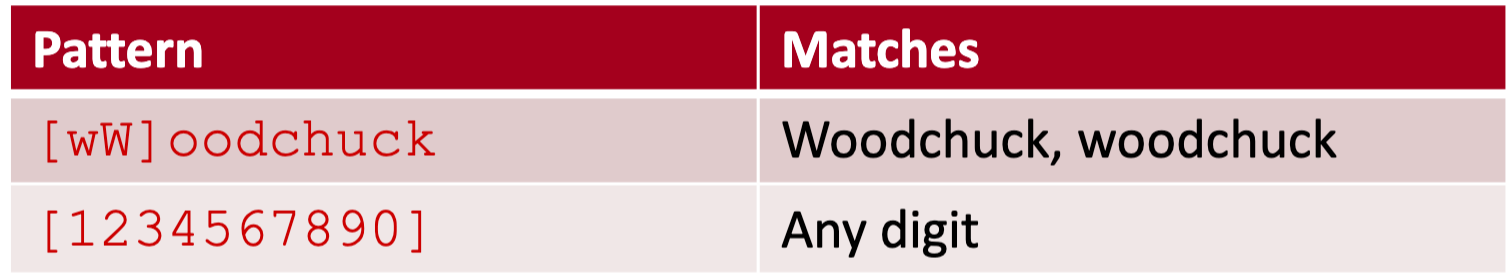
\includegraphics[width=\textwidth]{7.png}

Ranges [A-Z]

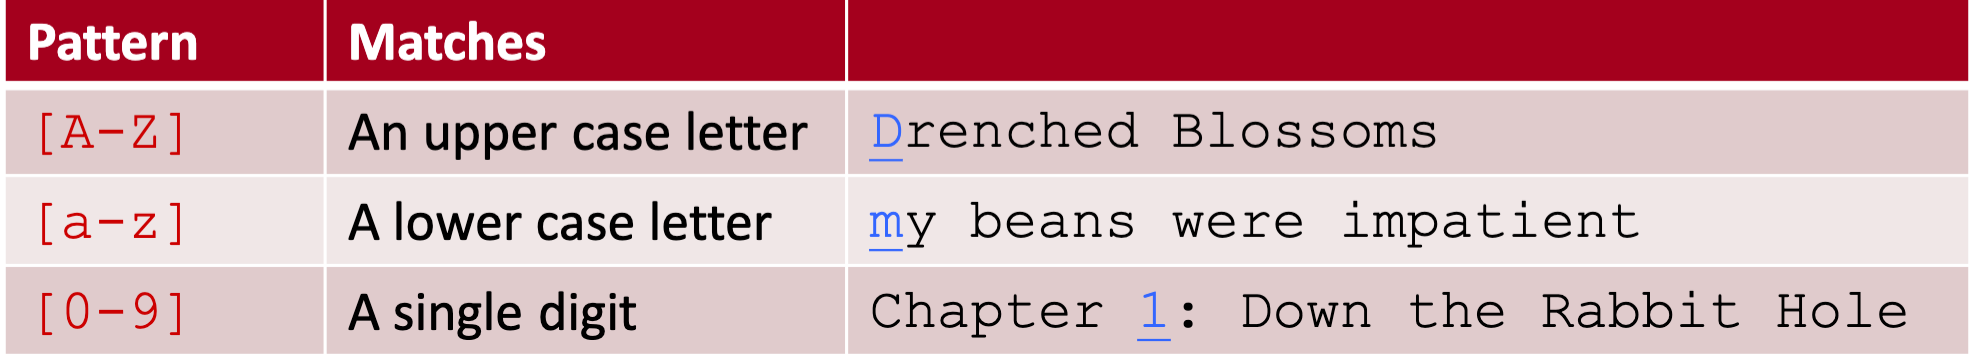
\includegraphics[width=\textwidth]{8.png}

\subsection{Regular Expressions: Negation in Disjunction}
Negations [\^Ss]

Carat means negation only when first in []

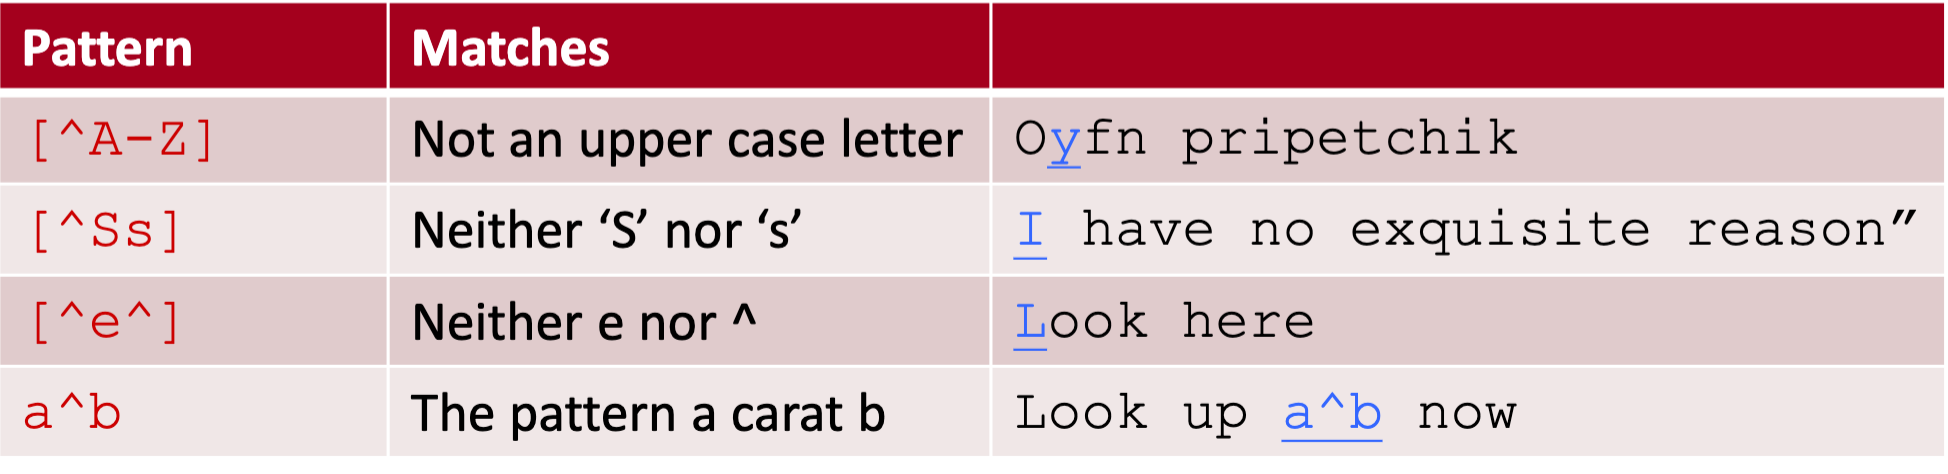
\includegraphics[width=\textwidth]{9.png}

\subsection{Regular Expressions: More Disjunction}
Woodchucks is another name for groundhog! The pipe | for disjunction.

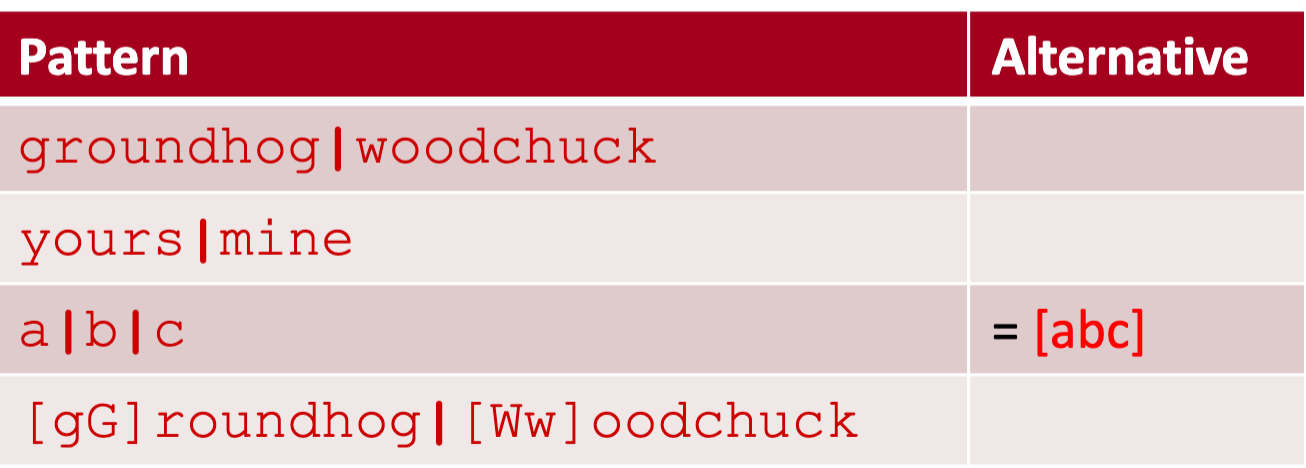
\includegraphics[width=\textwidth]{10.png}

\subsection{Regular Expressions: ? * + .}
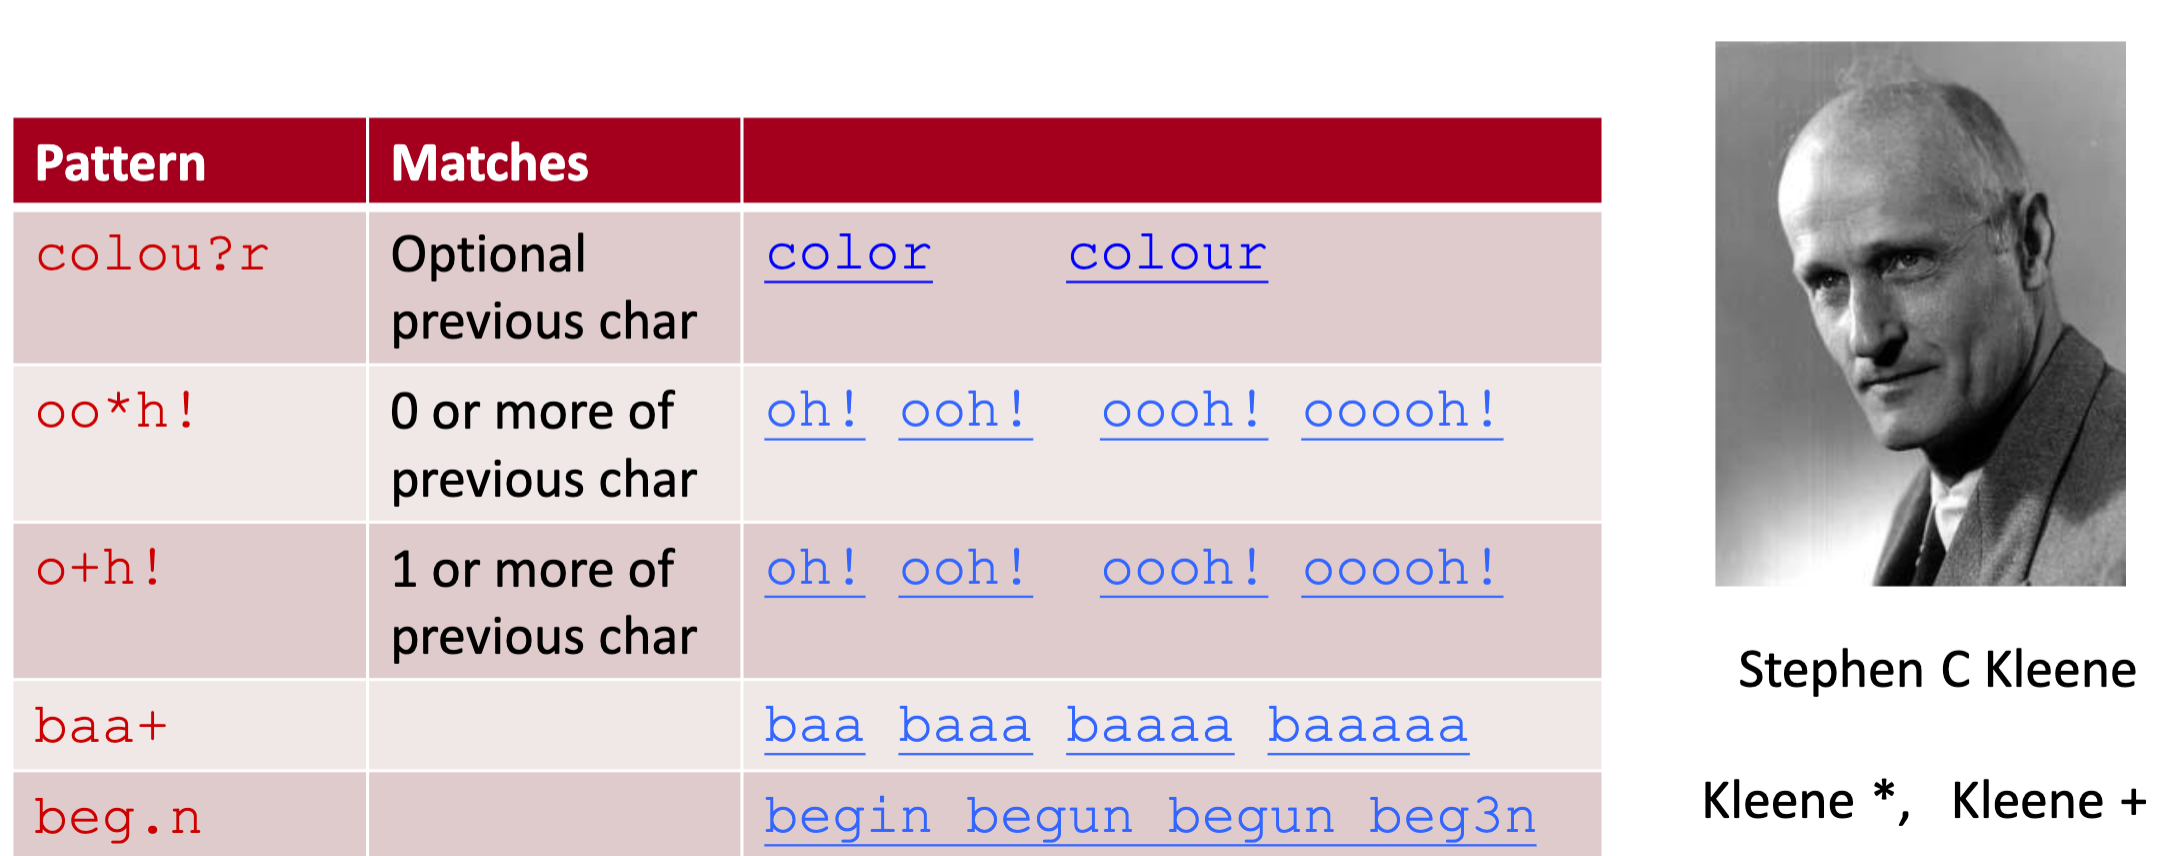
\includegraphics[width=\textwidth]{11.png}

\subsection{Regular Expressions: Anchors: \^ \$}
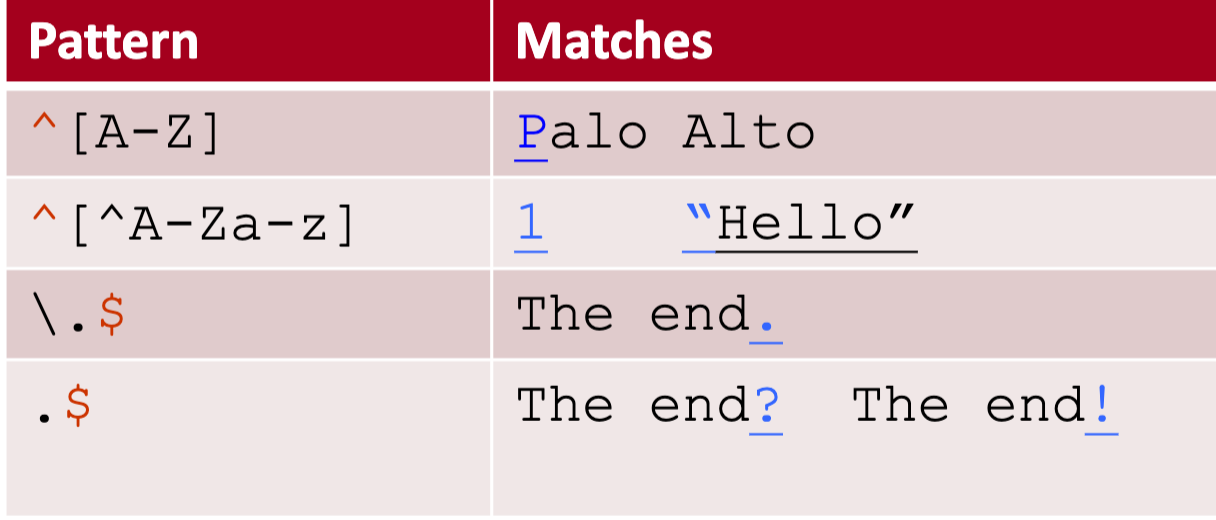
\includegraphics[width=\textwidth]{12.png}

\subsection{Example}
Find me all instances of the word “the” in a text.

the: Misses capitalized examples

[tT]he: Incorrectly returns other or theology

[\^a-zA-Z][tT]he[\^a-zA-Z]

\subsection{Exercise}
\begin{itemize}
  \item Write a regular expression to match dates
  \begin{itemize}
    \item November 9, 1989
    \item 17 December 1967
    \item 11-09-1989 (likely this form on midterm)
    \item 12/17/67
  \end{itemize}
  \item Write a regular expression to match time expressions
  \begin{itemize}
    \item Next Wednesday at noon
    \item Tomorrow morning
    \item Can't really as there's no general pattern
  \end{itemize}
\end{itemize}

\subsection{Errors}
\begin{itemize}
  \item The process we just went through was based on fixing
  two kinds of errors
  \begin{itemize}
    \item Matching strings that we should not have matched (there,
    then, other)
    \begin{itemize}
      \item False positives (Type I)
    \end{itemize}
    \item Not matching things that we should have matched (The)
    \begin{itemize}
      \item False negatives (Type II)
    \end{itemize}
  \end{itemize}
  \item In NLP we are always dealing with these kinds of
  errors.
  \item Reducing the error rate for an application often
  involves two antagonistic efforts:
  \begin{itemize}
    \item Increasing accuracy or precision (minimizing false positives)
    \item Increasing coverage or recall (minimizing false negatives).
  \end{itemize}
\end{itemize}

\subsection{Regex Summary}
\begin{itemize}
  \item Regular expressions play a surprisingly large role
  \begin{itemize}
    \item Sophisticated sequences of regular expressions are often the first model
    for any text processing text
  \end{itemize}
\end{itemize}
\begin{itemize}
  \item For many hard tasks, we use machine learning classifiers
  \begin{itemize}
    \item But regular expressions are used as features in the classifiers
    \item Can be very useful in capturing generalizations
  \end{itemize}
\end{itemize}
\end{document}